% Options for packages loaded elsewhere
\PassOptionsToPackage{unicode}{hyperref}
\PassOptionsToPackage{hyphens}{url}
\PassOptionsToPackage{dvipsnames,svgnames,x11names}{xcolor}
%
\documentclass[
  letterpaper,
  DIV=11,
  numbers=noendperiod]{scrartcl}

\usepackage{amsmath,amssymb}
\usepackage{iftex}
\ifPDFTeX
  \usepackage[T1]{fontenc}
  \usepackage[utf8]{inputenc}
  \usepackage{textcomp} % provide euro and other symbols
\else % if luatex or xetex
  \usepackage{unicode-math}
  \defaultfontfeatures{Scale=MatchLowercase}
  \defaultfontfeatures[\rmfamily]{Ligatures=TeX,Scale=1}
\fi
\usepackage{lmodern}
\ifPDFTeX\else  
    % xetex/luatex font selection
\fi
% Use upquote if available, for straight quotes in verbatim environments
\IfFileExists{upquote.sty}{\usepackage{upquote}}{}
\IfFileExists{microtype.sty}{% use microtype if available
  \usepackage[]{microtype}
  \UseMicrotypeSet[protrusion]{basicmath} % disable protrusion for tt fonts
}{}
\makeatletter
\@ifundefined{KOMAClassName}{% if non-KOMA class
  \IfFileExists{parskip.sty}{%
    \usepackage{parskip}
  }{% else
    \setlength{\parindent}{0pt}
    \setlength{\parskip}{6pt plus 2pt minus 1pt}}
}{% if KOMA class
  \KOMAoptions{parskip=half}}
\makeatother
\usepackage{xcolor}
\setlength{\emergencystretch}{3em} % prevent overfull lines
\setcounter{secnumdepth}{5}
% Make \paragraph and \subparagraph free-standing
\ifx\paragraph\undefined\else
  \let\oldparagraph\paragraph
  \renewcommand{\paragraph}[1]{\oldparagraph{#1}\mbox{}}
\fi
\ifx\subparagraph\undefined\else
  \let\oldsubparagraph\subparagraph
  \renewcommand{\subparagraph}[1]{\oldsubparagraph{#1}\mbox{}}
\fi

\usepackage{color}
\usepackage{fancyvrb}
\newcommand{\VerbBar}{|}
\newcommand{\VERB}{\Verb[commandchars=\\\{\}]}
\DefineVerbatimEnvironment{Highlighting}{Verbatim}{commandchars=\\\{\}}
% Add ',fontsize=\small' for more characters per line
\usepackage{framed}
\definecolor{shadecolor}{RGB}{241,243,245}
\newenvironment{Shaded}{\begin{snugshade}}{\end{snugshade}}
\newcommand{\AlertTok}[1]{\textcolor[rgb]{0.68,0.00,0.00}{#1}}
\newcommand{\AnnotationTok}[1]{\textcolor[rgb]{0.37,0.37,0.37}{#1}}
\newcommand{\AttributeTok}[1]{\textcolor[rgb]{0.40,0.45,0.13}{#1}}
\newcommand{\BaseNTok}[1]{\textcolor[rgb]{0.68,0.00,0.00}{#1}}
\newcommand{\BuiltInTok}[1]{\textcolor[rgb]{0.00,0.23,0.31}{#1}}
\newcommand{\CharTok}[1]{\textcolor[rgb]{0.13,0.47,0.30}{#1}}
\newcommand{\CommentTok}[1]{\textcolor[rgb]{0.37,0.37,0.37}{#1}}
\newcommand{\CommentVarTok}[1]{\textcolor[rgb]{0.37,0.37,0.37}{\textit{#1}}}
\newcommand{\ConstantTok}[1]{\textcolor[rgb]{0.56,0.35,0.01}{#1}}
\newcommand{\ControlFlowTok}[1]{\textcolor[rgb]{0.00,0.23,0.31}{#1}}
\newcommand{\DataTypeTok}[1]{\textcolor[rgb]{0.68,0.00,0.00}{#1}}
\newcommand{\DecValTok}[1]{\textcolor[rgb]{0.68,0.00,0.00}{#1}}
\newcommand{\DocumentationTok}[1]{\textcolor[rgb]{0.37,0.37,0.37}{\textit{#1}}}
\newcommand{\ErrorTok}[1]{\textcolor[rgb]{0.68,0.00,0.00}{#1}}
\newcommand{\ExtensionTok}[1]{\textcolor[rgb]{0.00,0.23,0.31}{#1}}
\newcommand{\FloatTok}[1]{\textcolor[rgb]{0.68,0.00,0.00}{#1}}
\newcommand{\FunctionTok}[1]{\textcolor[rgb]{0.28,0.35,0.67}{#1}}
\newcommand{\ImportTok}[1]{\textcolor[rgb]{0.00,0.46,0.62}{#1}}
\newcommand{\InformationTok}[1]{\textcolor[rgb]{0.37,0.37,0.37}{#1}}
\newcommand{\KeywordTok}[1]{\textcolor[rgb]{0.00,0.23,0.31}{#1}}
\newcommand{\NormalTok}[1]{\textcolor[rgb]{0.00,0.23,0.31}{#1}}
\newcommand{\OperatorTok}[1]{\textcolor[rgb]{0.37,0.37,0.37}{#1}}
\newcommand{\OtherTok}[1]{\textcolor[rgb]{0.00,0.23,0.31}{#1}}
\newcommand{\PreprocessorTok}[1]{\textcolor[rgb]{0.68,0.00,0.00}{#1}}
\newcommand{\RegionMarkerTok}[1]{\textcolor[rgb]{0.00,0.23,0.31}{#1}}
\newcommand{\SpecialCharTok}[1]{\textcolor[rgb]{0.37,0.37,0.37}{#1}}
\newcommand{\SpecialStringTok}[1]{\textcolor[rgb]{0.13,0.47,0.30}{#1}}
\newcommand{\StringTok}[1]{\textcolor[rgb]{0.13,0.47,0.30}{#1}}
\newcommand{\VariableTok}[1]{\textcolor[rgb]{0.07,0.07,0.07}{#1}}
\newcommand{\VerbatimStringTok}[1]{\textcolor[rgb]{0.13,0.47,0.30}{#1}}
\newcommand{\WarningTok}[1]{\textcolor[rgb]{0.37,0.37,0.37}{\textit{#1}}}

\providecommand{\tightlist}{%
  \setlength{\itemsep}{0pt}\setlength{\parskip}{0pt}}\usepackage{longtable,booktabs,array}
\usepackage{calc} % for calculating minipage widths
% Correct order of tables after \paragraph or \subparagraph
\usepackage{etoolbox}
\makeatletter
\patchcmd\longtable{\par}{\if@noskipsec\mbox{}\fi\par}{}{}
\makeatother
% Allow footnotes in longtable head/foot
\IfFileExists{footnotehyper.sty}{\usepackage{footnotehyper}}{\usepackage{footnote}}
\makesavenoteenv{longtable}
\usepackage{graphicx}
\makeatletter
\def\maxwidth{\ifdim\Gin@nat@width>\linewidth\linewidth\else\Gin@nat@width\fi}
\def\maxheight{\ifdim\Gin@nat@height>\textheight\textheight\else\Gin@nat@height\fi}
\makeatother
% Scale images if necessary, so that they will not overflow the page
% margins by default, and it is still possible to overwrite the defaults
% using explicit options in \includegraphics[width, height, ...]{}
\setkeys{Gin}{width=\maxwidth,height=\maxheight,keepaspectratio}
% Set default figure placement to htbp
\makeatletter
\def\fps@figure{htbp}
\makeatother

\KOMAoption{captions}{tableheading}
\makeatletter
\@ifpackageloaded{caption}{}{\usepackage{caption}}
\AtBeginDocument{%
\ifdefined\contentsname
  \renewcommand*\contentsname{Table of contents}
\else
  \newcommand\contentsname{Table of contents}
\fi
\ifdefined\listfigurename
  \renewcommand*\listfigurename{List of Figures}
\else
  \newcommand\listfigurename{List of Figures}
\fi
\ifdefined\listtablename
  \renewcommand*\listtablename{List of Tables}
\else
  \newcommand\listtablename{List of Tables}
\fi
\ifdefined\figurename
  \renewcommand*\figurename{Figure}
\else
  \newcommand\figurename{Figure}
\fi
\ifdefined\tablename
  \renewcommand*\tablename{Table}
\else
  \newcommand\tablename{Table}
\fi
}
\@ifpackageloaded{float}{}{\usepackage{float}}
\floatstyle{ruled}
\@ifundefined{c@chapter}{\newfloat{codelisting}{h}{lop}}{\newfloat{codelisting}{h}{lop}[chapter]}
\floatname{codelisting}{Listing}
\newcommand*\listoflistings{\listof{codelisting}{List of Listings}}
\makeatother
\makeatletter
\makeatother
\makeatletter
\@ifpackageloaded{caption}{}{\usepackage{caption}}
\@ifpackageloaded{subcaption}{}{\usepackage{subcaption}}
\makeatother
\ifLuaTeX
  \usepackage{selnolig}  % disable illegal ligatures
\fi
\usepackage{bookmark}

\IfFileExists{xurl.sty}{\usepackage{xurl}}{} % add URL line breaks if available
\urlstyle{same} % disable monospaced font for URLs
\hypersetup{
  pdftitle={EDA-challenge},
  pdfauthor={Erika Carlson},
  colorlinks=true,
  linkcolor={blue},
  filecolor={Maroon},
  citecolor={Blue},
  urlcolor={Blue},
  pdfcreator={LaTeX via pandoc}}

\title{EDA-challenge}
\author{Erika Carlson}
\date{2024-02-07}

\begin{document}
\maketitle

\renewcommand*\contentsname{Table of contents}
{
\hypersetup{linkcolor=}
\setcounter{tocdepth}{3}
\tableofcontents
}
\section{Explore and Wrangle Data}\label{explore-and-wrangle-data}

Load the ``data-wrangling.csv'' dataset from
\href{https://raw.githubusercontent.com/difiore/ada-2024-datasets/main/data-wrangling.csv}{\textbf{this
URL}} as a tabular data structure named \textbf{d} and look at the
variables it contains

\begin{Shaded}
\begin{Highlighting}[]
\FunctionTok{library}\NormalTok{(tidyverse)}
\end{Highlighting}
\end{Shaded}

\begin{verbatim}
Warning: package 'readr' was built under R version 4.2.3
\end{verbatim}

\begin{verbatim}
Warning: package 'dplyr' was built under R version 4.2.3
\end{verbatim}

\begin{verbatim}
Warning: package 'stringr' was built under R version 4.2.3
\end{verbatim}

\begin{verbatim}
-- Attaching core tidyverse packages ------------------------ tidyverse 2.0.0 --
v dplyr     1.1.4     v readr     2.1.5
v forcats   1.0.0     v stringr   1.5.1
v ggplot2   3.4.4     v tibble    3.2.1
v lubridate 1.9.3     v tidyr     1.3.0
v purrr     1.0.2     
-- Conflicts ------------------------------------------ tidyverse_conflicts() --
x dplyr::filter() masks stats::filter()
x dplyr::lag()    masks stats::lag()
i Use the conflicted package (<http://conflicted.r-lib.org/>) to force all conflicts to become errors
\end{verbatim}

\begin{Shaded}
\begin{Highlighting}[]
\NormalTok{f }\OtherTok{\textless{}{-}} \StringTok{"https://raw.githubusercontent.com/difiore/ada{-}2024{-}datasets/main/data{-}wrangling.csv"}
\NormalTok{d }\OtherTok{\textless{}{-}} \FunctionTok{read\_csv}\NormalTok{(f, }\AttributeTok{col\_names =} \ConstantTok{TRUE}\NormalTok{)}
\end{Highlighting}
\end{Shaded}

\begin{verbatim}
Rows: 213 Columns: 23
-- Column specification --------------------------------------------------------
Delimiter: ","
chr  (6): Scientific_Name, Family, Genus, Species, Leaves, Fauna
dbl (17): Brain_Size_Species_Mean, Body_mass_male_mean, Body_mass_female_mea...

i Use `spec()` to retrieve the full column specification for this data.
i Specify the column types or set `show_col_types = FALSE` to quiet this message.
\end{verbatim}

\begin{Shaded}
\begin{Highlighting}[]
\FunctionTok{names}\NormalTok{(d)}
\end{Highlighting}
\end{Shaded}

\begin{verbatim}
 [1] "Scientific_Name"         "Family"                 
 [3] "Genus"                   "Species"                
 [5] "Brain_Size_Species_Mean" "Body_mass_male_mean"    
 [7] "Body_mass_female_mean"   "MeanGroupSize"          
 [9] "AdultMales"              "AdultFemale"            
[11] "GR_MidRangeLat_dd"       "Precip_Mean_mm"         
[13] "Temp_Mean_degC"          "HomeRange_km2"          
[15] "DayLength_km"            "Fruit"                  
[17] "Leaves"                  "Fauna"                  
[19] "Canine_Dimorphism"       "Feed"                   
[21] "Move"                    "Rest"                   
[23] "Social"                 
\end{verbatim}

Create new variables - \textbf{BSD} (body size dimorphism), the ratio of
mean male to female body mass - \textbf{sex\_ratio}, the ratio of the
number of adult females to adult males in a typical group - \textbf{DI}
(for ``defensibility index''), the ratio of day range length to the
diameter of the home range

\begin{Shaded}
\begin{Highlighting}[]
\NormalTok{d }\OtherTok{\textless{}{-}}\NormalTok{ d }\SpecialCharTok{\%\textgreater{}\%} 
  \FunctionTok{mutate}\NormalTok{(}\AttributeTok{BSD =}\NormalTok{ Body\_mass\_male\_mean}\SpecialCharTok{/}\NormalTok{Body\_mass\_female\_mean, }
         \AttributeTok{sex\_ratio =}\NormalTok{ AdultFemale}\SpecialCharTok{/}\NormalTok{AdultMales,}
         \AttributeTok{DI =}\NormalTok{ DayLength\_km}\SpecialCharTok{/}\NormalTok{(}\FunctionTok{sqrt}\NormalTok{(HomeRange\_km2}\SpecialCharTok{/}\NormalTok{pi)}\SpecialCharTok{*}\DecValTok{2}\NormalTok{)) }\CommentTok{\# sqrt(Area/pi)*2 = d}
\end{Highlighting}
\end{Shaded}

Plot the relationship between \textbf{day range length} and \textbf{time
spent moving}, for these primate species overall and by family. - Do
species that spend more time moving travel farther overall? \emph{A:
Yes, based on regression line} - How about within any particular primate
family? \emph{A: Yes for Atelidae, Hylobatidae, Cebidae} - Should you
transform either of these variables? \emph{A: log transformed day range
length}

\begin{Shaded}
\begin{Highlighting}[]
\FunctionTok{library}\NormalTok{(ggplot2)}
\FunctionTok{library}\NormalTok{(cowplot) }\CommentTok{\# to show graphs side by side}
\end{Highlighting}
\end{Shaded}

\begin{verbatim}
Warning: package 'cowplot' was built under R version 4.2.3
\end{verbatim}

\begin{verbatim}

Attaching package: 'cowplot'
\end{verbatim}

\begin{verbatim}
The following object is masked from 'package:lubridate':

    stamp
\end{verbatim}

\begin{Shaded}
\begin{Highlighting}[]
\NormalTok{plot1 }\OtherTok{\textless{}{-}} \FunctionTok{ggplot}\NormalTok{(}\AttributeTok{data =}\NormalTok{ d, }
            \FunctionTok{aes}\NormalTok{(}\AttributeTok{x =} \FunctionTok{log}\NormalTok{(DayLength\_km), }
                \AttributeTok{y =}\NormalTok{ Move)) }\SpecialCharTok{+}  \CommentTok{\# build a plot object}
  \FunctionTok{xlab}\NormalTok{(}\StringTok{"log(Day range length)"}\NormalTok{) }\SpecialCharTok{+} \FunctionTok{ylab}\NormalTok{(}\StringTok{"Time spent moving"}\NormalTok{) }\SpecialCharTok{+} \CommentTok{\# modify the axis labels}
  \FunctionTok{geom\_point}\NormalTok{(}\AttributeTok{na.rm =} \ConstantTok{TRUE}\NormalTok{) }\SpecialCharTok{+} \CommentTok{\# make a scatterplot}
  \FunctionTok{geom\_smooth}\NormalTok{(}\AttributeTok{method =} \StringTok{"lm"}\NormalTok{, }\AttributeTok{na.rm =} \ConstantTok{TRUE}\NormalTok{) }\SpecialCharTok{+} \CommentTok{\# add a regression line}
  \FunctionTok{ylim}\NormalTok{(}\DecValTok{0}\NormalTok{, }\DecValTok{40}\NormalTok{) }\SpecialCharTok{+} \CommentTok{\# set y{-}axis range}
  \FunctionTok{theme}\NormalTok{(}\AttributeTok{legend.title =} \FunctionTok{element\_blank}\NormalTok{()) }\CommentTok{\# modify the legend}
\NormalTok{plot1 }\CommentTok{\# plot the object}
\end{Highlighting}
\end{Shaded}

\begin{verbatim}
`geom_smooth()` using formula = 'y ~ x'
\end{verbatim}

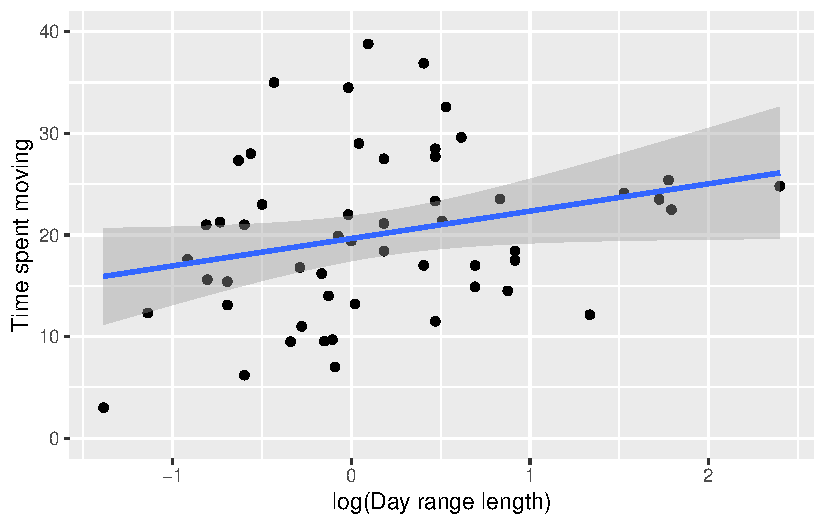
\includegraphics{EDA-challenge_files/figure-pdf/unnamed-chunk-3-1.pdf}

\begin{Shaded}
\begin{Highlighting}[]
\NormalTok{plot2 }\OtherTok{\textless{}{-}} \FunctionTok{ggplot}\NormalTok{(}\AttributeTok{data =}\NormalTok{ d, }
            \FunctionTok{aes}\NormalTok{(}\AttributeTok{x =} \FunctionTok{log}\NormalTok{(DayLength\_km), }
                \AttributeTok{y =}\NormalTok{ Move,}
                \AttributeTok{color =} \FunctionTok{factor}\NormalTok{(Family))) }\SpecialCharTok{+}  \CommentTok{\# build a plot object and color points by Family}
  \FunctionTok{xlab}\NormalTok{(}\StringTok{"log(Day range length)"}\NormalTok{) }\SpecialCharTok{+} \FunctionTok{ylab}\NormalTok{(}\StringTok{"Time spent moving"}\NormalTok{) }\SpecialCharTok{+} \CommentTok{\# modify the axis labels}
  \FunctionTok{geom\_point}\NormalTok{(}\AttributeTok{na.rm =} \ConstantTok{TRUE}\NormalTok{) }\SpecialCharTok{+} \CommentTok{\# make a scatterplot}
  \FunctionTok{geom\_smooth}\NormalTok{(}\AttributeTok{method =} \StringTok{"lm"}\NormalTok{, }\AttributeTok{na.rm =} \ConstantTok{TRUE}\NormalTok{) }\SpecialCharTok{+} \CommentTok{\# add a regression line}
  \FunctionTok{ylim}\NormalTok{(}\DecValTok{0}\NormalTok{, }\DecValTok{40}\NormalTok{) }\SpecialCharTok{+} \CommentTok{\# set y{-}axis range}
  \FunctionTok{theme}\NormalTok{(}\AttributeTok{legend.title =} \FunctionTok{element\_blank}\NormalTok{()) }\CommentTok{\# modify the legend}
\NormalTok{plot2 }\CommentTok{\# plot the object}
\end{Highlighting}
\end{Shaded}

\begin{verbatim}
`geom_smooth()` using formula = 'y ~ x'
\end{verbatim}

\begin{verbatim}
Warning in qt((1 - level)/2, df): NaNs produced
\end{verbatim}

\begin{verbatim}
Warning in max(ids, na.rm = TRUE): no non-missing arguments to max; returning
-Inf
\end{verbatim}

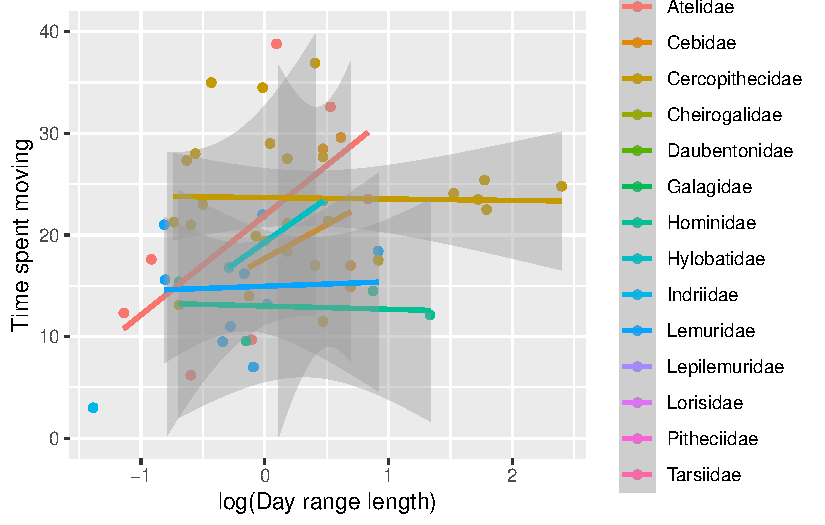
\includegraphics{EDA-challenge_files/figure-pdf/unnamed-chunk-3-2.pdf}

\begin{Shaded}
\begin{Highlighting}[]
\FunctionTok{plot\_grid}\NormalTok{(plot1, plot2, }\AttributeTok{rel\_widths =} \FunctionTok{c}\NormalTok{(}\DecValTok{1}\NormalTok{, }\FloatTok{1.5}\NormalTok{), }\AttributeTok{labels =} \StringTok{"AUTO"}\NormalTok{)}
\end{Highlighting}
\end{Shaded}

\begin{verbatim}
`geom_smooth()` using formula = 'y ~ x'
\end{verbatim}

\begin{verbatim}
`geom_smooth()` using formula = 'y ~ x'
\end{verbatim}

\begin{verbatim}
Warning in qt((1 - level)/2, df): NaNs produced

Warning in qt((1 - level)/2, df): no non-missing arguments to max; returning
-Inf
\end{verbatim}

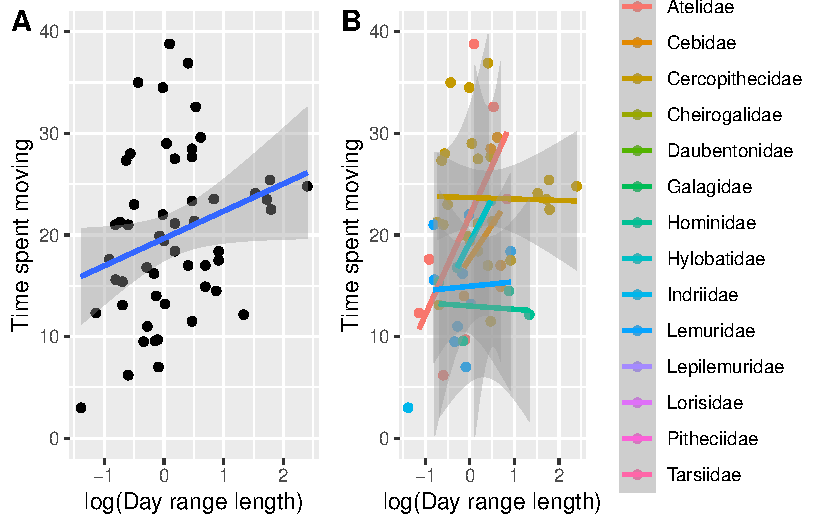
\includegraphics{EDA-challenge_files/figure-pdf/unnamed-chunk-3-3.pdf}

Plot the relationship between \textbf{day range length} and \textbf{mean
group size}, overall and by family. - Do species that live in larger
groups travel farther overall? \emph{A: Yes, based on regression line} -
How about within any particular primate family? \emph{A: Yes for
Cercopithecidae, Hominidae, Tarsiidae, Cebidae} - Should you transform
either of these variables? \emph{A: log transformed day range length}

\begin{Shaded}
\begin{Highlighting}[]
\NormalTok{plot1 }\OtherTok{\textless{}{-}} \FunctionTok{ggplot}\NormalTok{(}\AttributeTok{data =}\NormalTok{ d, }
            \FunctionTok{aes}\NormalTok{(}\AttributeTok{x =} \FunctionTok{log}\NormalTok{(DayLength\_km), }
                \AttributeTok{y =}\NormalTok{ MeanGroupSize)) }\SpecialCharTok{+}  \CommentTok{\# build a plot object}
  \FunctionTok{xlab}\NormalTok{(}\StringTok{"log(Day range length)"}\NormalTok{) }\SpecialCharTok{+} \FunctionTok{ylab}\NormalTok{(}\StringTok{"Group Size"}\NormalTok{) }\SpecialCharTok{+} \CommentTok{\# modify the axis labels}
  \FunctionTok{geom\_point}\NormalTok{(}\AttributeTok{na.rm =} \ConstantTok{TRUE}\NormalTok{) }\SpecialCharTok{+} \CommentTok{\# make a scatterplot}
  \FunctionTok{geom\_smooth}\NormalTok{(}\AttributeTok{method =} \StringTok{"lm"}\NormalTok{, }\AttributeTok{na.rm =} \ConstantTok{TRUE}\NormalTok{) }\SpecialCharTok{+} \CommentTok{\# add a regression line}
  \FunctionTok{ylim}\NormalTok{(}\DecValTok{0}\NormalTok{, }\DecValTok{100}\NormalTok{) }\SpecialCharTok{+} \CommentTok{\# set y{-}axis range}
  \FunctionTok{theme}\NormalTok{(}\AttributeTok{legend.title =} \FunctionTok{element\_blank}\NormalTok{()) }\CommentTok{\# modify the legend}
\NormalTok{plot1 }\CommentTok{\# plot the object}
\end{Highlighting}
\end{Shaded}

\begin{verbatim}
`geom_smooth()` using formula = 'y ~ x'
\end{verbatim}

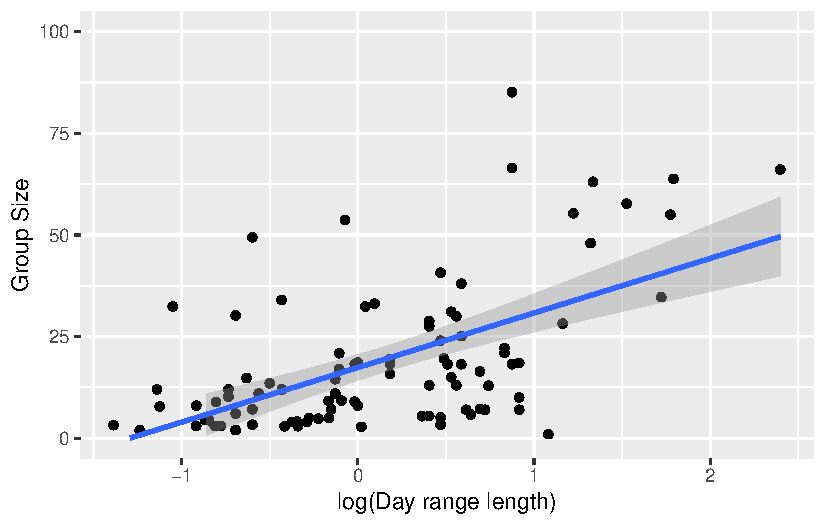
\includegraphics{EDA-challenge_files/figure-pdf/unnamed-chunk-4-1.pdf}

\begin{Shaded}
\begin{Highlighting}[]
\NormalTok{plot2 }\OtherTok{\textless{}{-}} \FunctionTok{ggplot}\NormalTok{(}\AttributeTok{data =}\NormalTok{ d, }
            \FunctionTok{aes}\NormalTok{(}\AttributeTok{x =} \FunctionTok{log}\NormalTok{(DayLength\_km), }
                \AttributeTok{y =}\NormalTok{ MeanGroupSize,}
                \AttributeTok{color =} \FunctionTok{factor}\NormalTok{(Family))) }\SpecialCharTok{+}  \CommentTok{\# build a plot object and color points by Family}
  \FunctionTok{xlab}\NormalTok{(}\StringTok{"log(Day range length)"}\NormalTok{) }\SpecialCharTok{+} \FunctionTok{ylab}\NormalTok{(}\StringTok{"Group Size"}\NormalTok{) }\SpecialCharTok{+} \CommentTok{\# modify the axis labels}
  \FunctionTok{geom\_point}\NormalTok{(}\AttributeTok{na.rm =} \ConstantTok{TRUE}\NormalTok{) }\SpecialCharTok{+} \CommentTok{\# make a scatterplot}
  \FunctionTok{geom\_smooth}\NormalTok{(}\AttributeTok{method =} \StringTok{"lm"}\NormalTok{, }\AttributeTok{na.rm =} \ConstantTok{TRUE}\NormalTok{) }\SpecialCharTok{+} \CommentTok{\# add a regression line}
  \FunctionTok{ylim}\NormalTok{(}\DecValTok{0}\NormalTok{, }\DecValTok{100}\NormalTok{) }\SpecialCharTok{+} \CommentTok{\# set y{-}axis range}
  \FunctionTok{theme}\NormalTok{(}\AttributeTok{legend.title =} \FunctionTok{element\_blank}\NormalTok{()) }\CommentTok{\# modify the legend}
\NormalTok{plot2 }\CommentTok{\# plot the object}
\end{Highlighting}
\end{Shaded}

\begin{verbatim}
`geom_smooth()` using formula = 'y ~ x'
\end{verbatim}

\begin{verbatim}
Warning in qt((1 - level)/2, df): NaNs produced
\end{verbatim}

\begin{verbatim}
Warning in max(ids, na.rm = TRUE): no non-missing arguments to max; returning
-Inf

Warning in max(ids, na.rm = TRUE): no non-missing arguments to max; returning
-Inf

Warning in max(ids, na.rm = TRUE): no non-missing arguments to max; returning
-Inf
\end{verbatim}

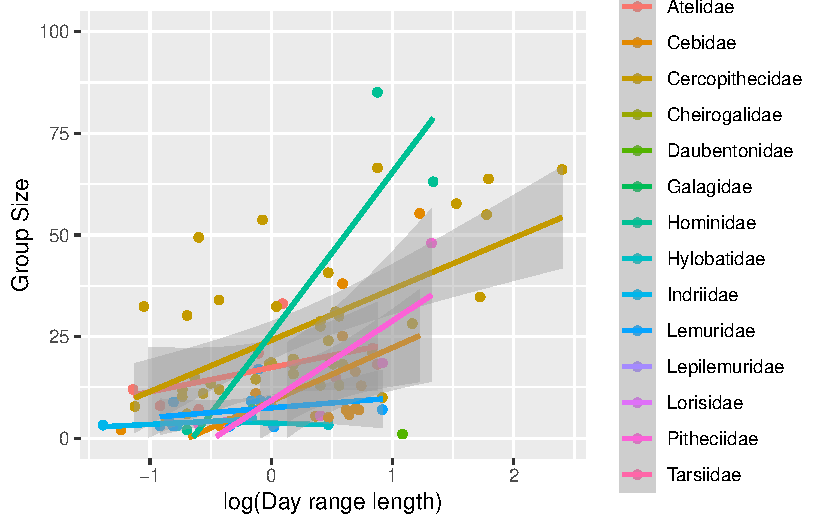
\includegraphics{EDA-challenge_files/figure-pdf/unnamed-chunk-4-2.pdf}

\begin{Shaded}
\begin{Highlighting}[]
\FunctionTok{plot\_grid}\NormalTok{(plot1, plot2, }\AttributeTok{rel\_widths =} \FunctionTok{c}\NormalTok{(}\DecValTok{1}\NormalTok{, }\FloatTok{1.5}\NormalTok{), }\AttributeTok{labels =} \StringTok{"AUTO"}\NormalTok{)}
\end{Highlighting}
\end{Shaded}

\begin{verbatim}
`geom_smooth()` using formula = 'y ~ x'
`geom_smooth()` using formula = 'y ~ x'
\end{verbatim}

\begin{verbatim}
Warning in qt((1 - level)/2, df): NaNs produced

Warning in qt((1 - level)/2, df): no non-missing arguments to max; returning
-Inf

Warning in qt((1 - level)/2, df): no non-missing arguments to max; returning
-Inf

Warning in qt((1 - level)/2, df): no non-missing arguments to max; returning
-Inf
\end{verbatim}

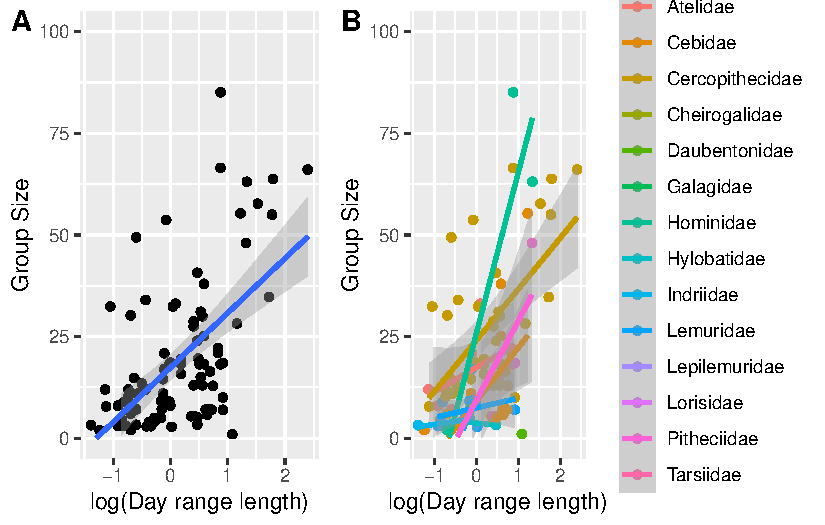
\includegraphics{EDA-challenge_files/figure-pdf/unnamed-chunk-4-3.pdf}

Plot the relationship between \textbf{body size dimorphism} and
\textbf{canine size dimorphism} overall and by family.

Do taxa with greater size dimorphism also show greater canine
dimorphism? \emph{A: Yes, overall and in Carcopithecidae, Hominidae,
Cebidae, Tarsiidae, and Lorisidae families}

\begin{Shaded}
\begin{Highlighting}[]
\NormalTok{plot1 }\OtherTok{\textless{}{-}} \FunctionTok{ggplot}\NormalTok{(}\AttributeTok{data =}\NormalTok{ d, }
            \FunctionTok{aes}\NormalTok{(}\AttributeTok{x =}\NormalTok{ BSD, }
                \AttributeTok{y =}\NormalTok{ Canine\_Dimorphism)) }\SpecialCharTok{+}  \CommentTok{\# build a plot object}
  \FunctionTok{xlab}\NormalTok{(}\StringTok{"Body size dimorphism"}\NormalTok{) }\SpecialCharTok{+} \FunctionTok{ylab}\NormalTok{(}\StringTok{"Canine size dimorphism"}\NormalTok{) }\SpecialCharTok{+} \CommentTok{\# modify the axis labels}
  \FunctionTok{geom\_point}\NormalTok{(}\AttributeTok{na.rm =} \ConstantTok{TRUE}\NormalTok{) }\SpecialCharTok{+} \CommentTok{\# make a scatterplot}
  \FunctionTok{geom\_smooth}\NormalTok{(}\AttributeTok{method =} \StringTok{"lm"}\NormalTok{, }\AttributeTok{na.rm =} \ConstantTok{TRUE}\NormalTok{) }\SpecialCharTok{+} \CommentTok{\# add a regression line}
  \CommentTok{\# ylim(0, 100) + \# set y{-}axis range}
  \FunctionTok{theme}\NormalTok{(}\AttributeTok{legend.title =} \FunctionTok{element\_blank}\NormalTok{()) }\CommentTok{\# modify the legend}
\NormalTok{plot1 }\CommentTok{\# plot the object}
\end{Highlighting}
\end{Shaded}

\begin{verbatim}
`geom_smooth()` using formula = 'y ~ x'
\end{verbatim}

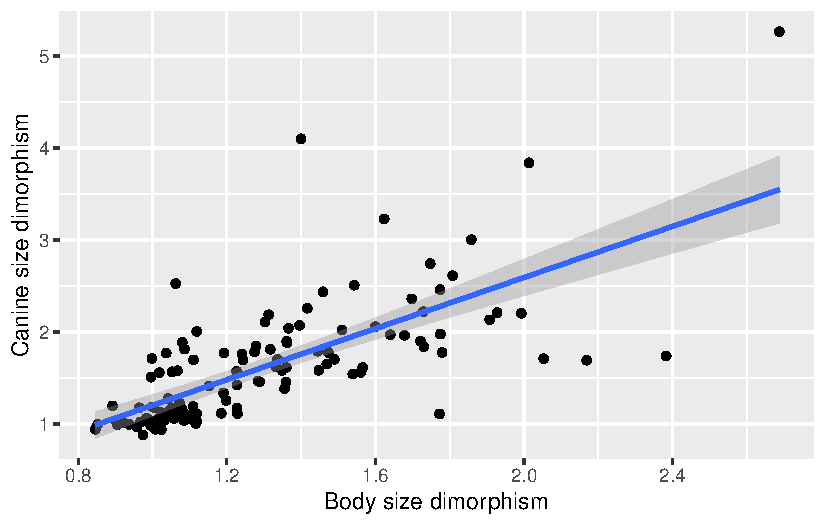
\includegraphics{EDA-challenge_files/figure-pdf/unnamed-chunk-5-1.pdf}

\begin{Shaded}
\begin{Highlighting}[]
\NormalTok{plot2 }\OtherTok{\textless{}{-}} \FunctionTok{ggplot}\NormalTok{(}\AttributeTok{data =}\NormalTok{ d, }
            \FunctionTok{aes}\NormalTok{(}\AttributeTok{x =}\NormalTok{ BSD, }
                \AttributeTok{y =}\NormalTok{ Canine\_Dimorphism,}
                \AttributeTok{color =} \FunctionTok{factor}\NormalTok{(Family))) }\SpecialCharTok{+}  \CommentTok{\# build a plot object and color points by Family}
  \FunctionTok{xlab}\NormalTok{(}\StringTok{"Body size dimorphism"}\NormalTok{) }\SpecialCharTok{+} \FunctionTok{ylab}\NormalTok{(}\StringTok{"Canine size dimorphism"}\NormalTok{) }\SpecialCharTok{+} \CommentTok{\# modify the axis labels}
  \FunctionTok{geom\_point}\NormalTok{(}\AttributeTok{na.rm =} \ConstantTok{TRUE}\NormalTok{) }\SpecialCharTok{+} \CommentTok{\# make a scatterplot}
  \FunctionTok{geom\_smooth}\NormalTok{(}\AttributeTok{method =} \StringTok{"lm"}\NormalTok{, }\AttributeTok{na.rm =} \ConstantTok{TRUE}\NormalTok{) }\SpecialCharTok{+} \CommentTok{\# add a regression line}
  \CommentTok{\# ylim(0, 100) + \# set y{-}axis range}
  \FunctionTok{theme}\NormalTok{(}\AttributeTok{legend.title =} \FunctionTok{element\_blank}\NormalTok{()) }\CommentTok{\# modify the legend}
\NormalTok{plot2 }\CommentTok{\# plot the object}
\end{Highlighting}
\end{Shaded}

\begin{verbatim}
`geom_smooth()` using formula = 'y ~ x'
\end{verbatim}

\begin{verbatim}
Warning in qt((1 - level)/2, df): NaNs produced
\end{verbatim}

\begin{verbatim}
Warning in max(ids, na.rm = TRUE): no non-missing arguments to max; returning
-Inf
\end{verbatim}

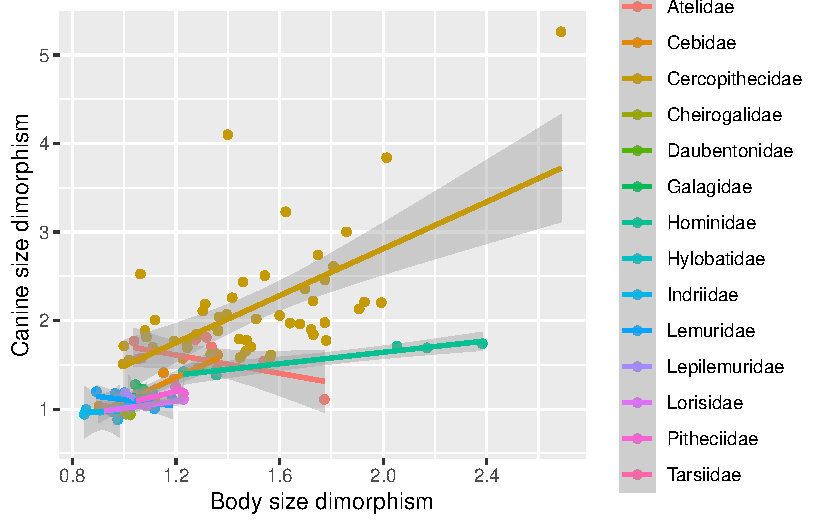
\includegraphics{EDA-challenge_files/figure-pdf/unnamed-chunk-5-2.pdf}

\begin{Shaded}
\begin{Highlighting}[]
\FunctionTok{plot\_grid}\NormalTok{(plot1, plot2, }\AttributeTok{rel\_widths =} \FunctionTok{c}\NormalTok{(}\DecValTok{1}\NormalTok{, }\FloatTok{1.5}\NormalTok{), }\AttributeTok{labels =} \StringTok{"AUTO"}\NormalTok{)}
\end{Highlighting}
\end{Shaded}

\begin{verbatim}
`geom_smooth()` using formula = 'y ~ x'
`geom_smooth()` using formula = 'y ~ x'
\end{verbatim}

\begin{verbatim}
Warning in qt((1 - level)/2, df): NaNs produced

Warning in qt((1 - level)/2, df): no non-missing arguments to max; returning
-Inf
\end{verbatim}

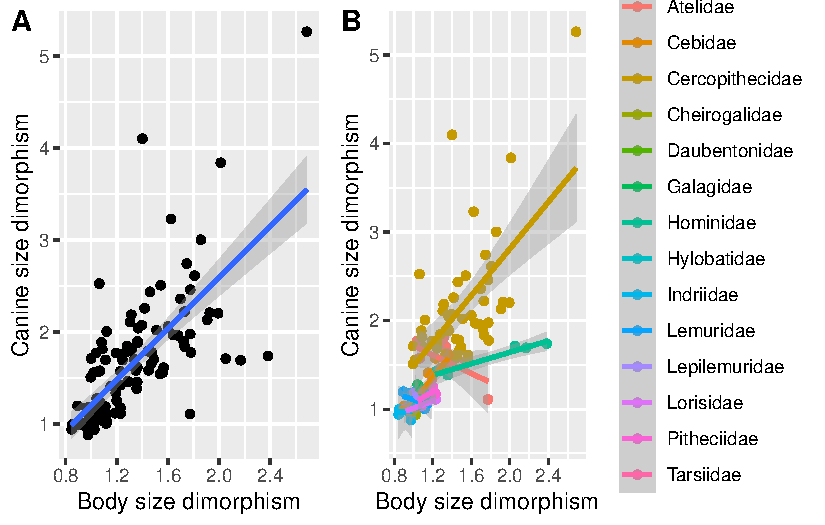
\includegraphics{EDA-challenge_files/figure-pdf/unnamed-chunk-5-3.pdf}

Create a new variable named diet\_strategy that is ``frugivore'' if
fruits make up \textgreater50\% of the diet, ``folivore'' if leaves make
up \textgreater50\% of the diet, and ``omnnivore'' if neither of these
is true. Then, do boxplots of group size for species with different
dietary strategies.

Do frugivores live in larger groups than folivores? \emph{A: No, overlap
in IQR (frugivore has more outliers)}

\begin{Shaded}
\begin{Highlighting}[]
\NormalTok{d }\OtherTok{\textless{}{-}}\NormalTok{ d }\SpecialCharTok{\%\textgreater{}\%} 
  \FunctionTok{mutate}\NormalTok{(}\AttributeTok{diet\_strategy =} \FunctionTok{case\_when}\NormalTok{(Fruit }\SpecialCharTok{\textgreater{}} \DecValTok{50} \SpecialCharTok{\textasciitilde{}} \StringTok{"frugivore"}\NormalTok{,}
\NormalTok{                                   Leaves }\SpecialCharTok{\textgreater{}} \DecValTok{50} \SpecialCharTok{\textasciitilde{}} \StringTok{"folivore"}\NormalTok{,}
\NormalTok{                                   Fruit }\SpecialCharTok{\textless{}} \DecValTok{50} \SpecialCharTok{\&}\NormalTok{ Leaves }\SpecialCharTok{\textless{}} \DecValTok{50} \SpecialCharTok{\textasciitilde{}} \StringTok{"omnivore"}\NormalTok{)) }\CommentTok{\# specify to avoid NAs}
\end{Highlighting}
\end{Shaded}

\begin{Shaded}
\begin{Highlighting}[]
\NormalTok{p }\OtherTok{\textless{}{-}} \FunctionTok{ggplot}\NormalTok{(}\AttributeTok{data =}\NormalTok{ d, }
            \FunctionTok{aes}\NormalTok{(}\AttributeTok{x =} \FunctionTok{factor}\NormalTok{(}\DecValTok{0}\NormalTok{), }\AttributeTok{y =}\NormalTok{ MeanGroupSize)) }\SpecialCharTok{+} 
  \FunctionTok{geom\_boxplot}\NormalTok{(}\AttributeTok{na.rm =} \ConstantTok{TRUE}\NormalTok{, }\AttributeTok{outlier.shape =} \ConstantTok{NA}\NormalTok{) }\SpecialCharTok{+} 
  \FunctionTok{theme}\NormalTok{(}\AttributeTok{axis.title.x =} \FunctionTok{element\_blank}\NormalTok{(), }
        \AttributeTok{axis.text.x =} \FunctionTok{element\_blank}\NormalTok{(), }
        \AttributeTok{axis.ticks.x =} \FunctionTok{element\_blank}\NormalTok{()) }\SpecialCharTok{+} 
  \FunctionTok{geom\_dotplot}\NormalTok{(}\AttributeTok{binaxis =} \StringTok{"y"}\NormalTok{, }\AttributeTok{stackdir =} \StringTok{"center"}\NormalTok{, }
               \AttributeTok{stackratio =} \FloatTok{0.2}\NormalTok{, }\AttributeTok{alpha =} \FloatTok{0.3}\NormalTok{, }\AttributeTok{dotsize =} \FloatTok{0.5}\NormalTok{, }\AttributeTok{color =} \ConstantTok{NA}\NormalTok{, }
               \AttributeTok{fill =} \StringTok{"blue"}\NormalTok{, }\AttributeTok{na.rm =} \ConstantTok{TRUE}\NormalTok{) }\SpecialCharTok{+}
  \FunctionTok{facet\_grid}\NormalTok{(. }\SpecialCharTok{\textasciitilde{}}\NormalTok{ diet\_strategy) }\SpecialCharTok{+} \FunctionTok{geom\_rug}\NormalTok{(}\AttributeTok{sides =} \StringTok{"l"}\NormalTok{)}
\NormalTok{p}
\end{Highlighting}
\end{Shaded}

\begin{verbatim}
Bin width defaults to 1/30 of the range of the data. Pick better value with
`binwidth`.
\end{verbatim}

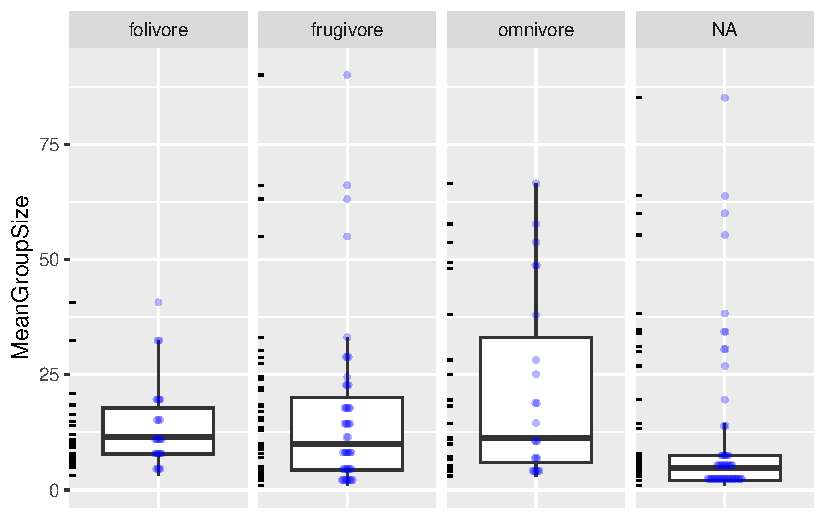
\includegraphics{EDA-challenge_files/figure-pdf/unnamed-chunk-7-1.pdf}

In one line of code, using \{dplyr\} verbs and the forward pipe
(\texttt{\%\textgreater{}\%} or \texttt{\textbar{}\textgreater{}})
operator, do the following: - Add a variable, \textbf{Binomial} to the
data frame \textbf{d}, which is a concatenation of the \textbf{Genus}
and \textbf{Species}\ldots{} - Trim the data frame to only include the
variables \textbf{Binomial}, \textbf{Family},
\textbf{Brain\_size\_species\_mean}, and
\textbf{Body\_mass\_male\_mean}\ldots{} - Group these variables by
\textbf{Family}\ldots{} - Calculate the average value for
\textbf{Brain\_size\_species\_mean} and \textbf{Body\_mass\_male\_mean}
per \textbf{Family} (remember, you may need to specify na.rm =
TRUE)\ldots{} - And arrange by increasing \textbf{average brain size}

\begin{Shaded}
\begin{Highlighting}[]
\NormalTok{d }\OtherTok{\textless{}{-}}\NormalTok{ d }\SpecialCharTok{\%\textgreater{}\%} 
  \FunctionTok{mutate}\NormalTok{(}\AttributeTok{Binomial =} \FunctionTok{str\_c}\NormalTok{(Genus, }\StringTok{" "}\NormalTok{, Species)) }\SpecialCharTok{\%\textgreater{}\%} 
  \FunctionTok{select}\NormalTok{(Binomial, Family, Brain\_Size\_Species\_Mean, Body\_mass\_male\_mean) }\SpecialCharTok{\%\textgreater{}\%} 
  \FunctionTok{group\_by}\NormalTok{(Family) }\SpecialCharTok{\%\textgreater{}\%} 
  \FunctionTok{summarize}\NormalTok{(}\AttributeTok{avg\_brain\_size =} \FunctionTok{mean}\NormalTok{(Brain\_Size\_Species\_Mean),}
            \AttributeTok{avg\_male\_body\_mass =} \FunctionTok{mean}\NormalTok{(Body\_mass\_male\_mean)) }\SpecialCharTok{\%\textgreater{}\%} 
  \FunctionTok{arrange}\NormalTok{(avg\_brain\_size)}
\end{Highlighting}
\end{Shaded}




\end{document}
